\documentclass[11pt]{article}
\usepackage[margin=1in, lmargin=0.75in]{geometry}
\usepackage{caption}
\usepackage{float}
\usepackage{graphicx}
\usepackage{latexsym}
\usepackage{amsmath}
\usepackage{cancel}
\usepackage{astro}
\usepackage{url}
\usepackage[bottom]{footmisc}

\newcommand\allbold[1]{{\boldmath\textbf{#1}}}
\newcommand\pc{\mathrm{\ pc}}
\newcommand\Lpc{\ L_\odot/\!\!\pc^2}
\newcommand\sech{\ \!\mathrm{sech}}
\newcommand\lsol{\mathrm{L}_\odot}
\newcommand\rsol{\mathrm{R}_\odot}
\newcommand\msol{\mathrm{M}_\odot}

\begin{document}

\begin{flushright}Meredith Durbin\\
Emily Levesque\\
Astro 531: Stellar Interiors\\
\today\\

\end{flushright}

\center{\textsc{Homework 1}} \\[6pt]

All calculations can be found in the notebook \url{https://github.com/meredith-durbin/ASTR531/blob/master/HW1/HW1.ipynb}.

% 2.3, 3.4, 4.3, 5.2, 6.2, and 7.3 

\begin{enumerate}

\item [2.3]
	\begin{enumerate}
	
    \item A distance of 470 ly gives $\tau$ Sco a distance modulus of 5.79 mag, which means that its $M_V$ is $-2.99$ mag.
    
    \item With a bolometric correction of $-3.16$ mag, the bolometric magnitude is $M_\mathrm{bol} = -6.15$ mag, giving a luminosity of $2.28 \times 10^4~\lsol$.
    
    \item From the Stefan-Boltzmann equation, the radius of the star is $5.59~\rsol$.

    \item Using the relation $\mathrm{L}/\lsol = 1.5(\mathrm{M}/\msol)^{3.5}$, we find a mass of $15.65~\msol$.
    
    \item The surface gravity of the star is $1.37 \times 10^4$ cm s$^{-2}$ ($\log g = 4.13$), and the escape velocity is $1.03 \times 10^8$ cm s$^{-1}$.
    
    \item The mean density is $\rho = 0.12$ g cm$^{-3}$.
    
    \item The surface gravity of $\tau$ Sco is about half that of the sun, whereas the escape velocity is about 1.67 times solar. $\tau$ Sco's mean density is only 0.09 of solar.
    
    \end{enumerate}

\item [3.4]
	% The virial theorem states that $-\Omega = 2U$.

\item [4.3]
    Based on the plot of solar temperature vs. density, it looks as though the sun is mostly in the ideal gas regime, and becomes degenerate at the highest densities.
	\begin{figure}[H]
	\centering
	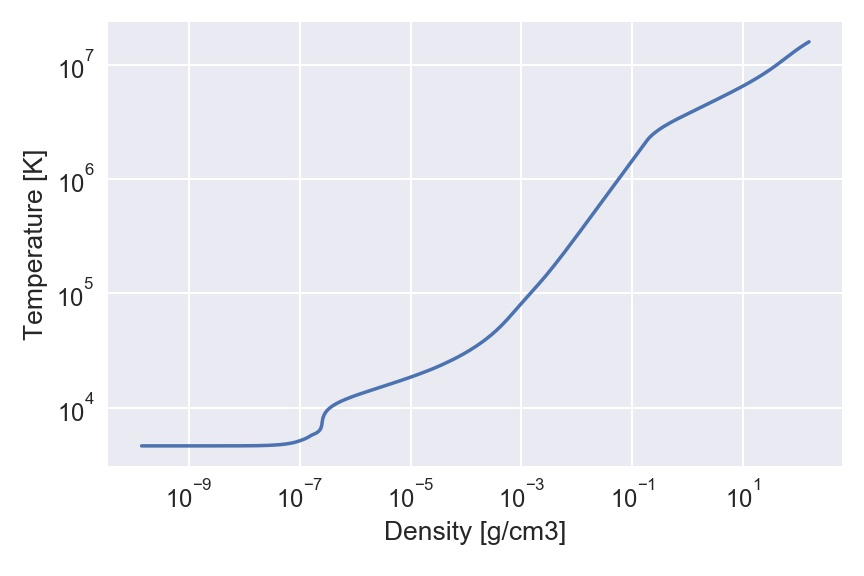
\includegraphics[width=0.6\textwidth]{temp_density.jpg}
	\end{figure}

\item [5.2]
	\begin{enumerate}
	
    \item For a mean free path of $\ell = 1$ cm, it will take a photon about $5 \times 10^{21}$ scatterings to travel $1~\rsol$.
    
    \item The total path length $\ell N$ is $5 \times 10^{21}$ cm, or $6.9 \times 10^{10}~\rsol$. It will take a photon traveling this path $1.6 \times 10^{11}$ s to exit the sun, or a little over 5000 years.
    
    \item This is almost certainly not the same photon.
    
    \end{enumerate}

\item [6.2]
	\begin{enumerate}
    \item 
    \end{enumerate}

\item [7.3]
	\begin{enumerate}
    \item The main sequence lifetime can be estimate by comparing the stellar luminosity to the total amount of energy that core fusion can produce. Assuming that all of the hydrogen in the convective core is converted to helium over the MS lifetime, and assuming a hydrogen fusion efficiency factor of 0.007, we can estimate the MS lifetime as $t_\mathrm{ms} = 0.007 M_\mathrm{core} c^2 / L_\star$. Assuming a convective core mass fraction of 0.25 for $4~\msol$ and 0.5 for $20~\msol$, we find MS lifetimes of $1.4 \times 10^{16}$ s and $8 \times 10^{14}$ s respectively, or $4.4 \times 10^{8}$ and $2.5 \times 10^{7}$ years.
    
    \item According to Appendix D, the MS lifetimes of 4 and $20~\msol$ stars are $1.5 \times 10^8$ and $7.8 \times 10^6$ years respectively. Our derived lifetimes are slight overestimates.
    % logL_zams, log t, logL_tams for 4. solmass star: 2.37, 8.18, 2.61
    % logL_zams, log t, logL_tams for 20 solmass star: 4.61, 6.89, 4.95
    \end{enumerate}


\end{enumerate}
\end{document}